\section{Moments of the point set}
\label{sec:moments}

By \Cref{lem:lines}(1) the origin is the centroid of the $N$ points for every arrangement, so the unweighted balance of the vectors $\mathbf p_{ij}$ carries no information about $S$.
The line conditions are statements about moments weighted by the heights.
Write $R_i=\sum_jz_{ij}$ and $C_j=\sum_iz_{ij}$ for the row and column deviations; $S$ is semi-magic if and only if all $R_i$ and $C_j$ vanish.

\paragraph{Row and column sums as moment conditions.}
For every function $\varphi\colon\R\to\R$, grouping the cells by column and by row gives
\begin{equation}
\sum_{i,j}z_{ij}\,\varphi(x_{ij})=\sum_j\varphi(x_j)\,C_j,\qquad
\sum_{i,j}z_{ij}\,\varphi(y_{ij})=\sum_i\varphi(y_i)\,R_i .
\label{eq:moments}
\end{equation}
Since the functions $\varphi(x)$ on the grid span the indicator functions of the columns, $S$ is semi-magic if and only if both sums vanish for every $\varphi$.
For $\varphi(t)=t$ this says that the \emph{dipole moment} $\sum z\,(x,y)$ of the signed masses $z_{ij}$ (total mass $0$) vanishes, in the multipole language of Rogers and Loly \cite{rogers2005multipole}; for $\varphi(t)=t^2$ it gives Loly's invariant below.
The diagonal conditions are not of this form.
The mixed moment $\sum z\,xy$ is not forced: over the $880$ order-four magic squares, $8\sum z\,xy$ takes $48$ distinct absolute values between $0$ and $480$ and vanishes for $56$ classes (\Cref{fig:moments}b, \Cref{fig:weighted}).
It vanishes whenever $S$ is associative, since then $z$ is odd under $(x,y)\mapsto(-x,-y)$; this accounts for $48$ of the $56$.

\begin{corollary}[Loly \cite{loly2004invariance}]
\label{cor:loly}
For every arrangement, $J(S):=\sum_{i,j}s_{ij}(x_{ij}^2+y_{ij}^2)=\sum_jx_j^2C_j+\sum_iy_i^2R_i+\frac{n^2(n^4-1)}{12}$; in particular $J(S)=n^2(n^4-1)/12$ for every semi-magic square.
\end{corollary}

\begin{proof}
Substitute $s_{ij}=z_{ij}+\bar s$, apply \eqref{eq:moments} with $\varphi(t)=t^2$ to the first part and \Cref{lem:lines}(2) to $\bar s\sum(x^2+y^2)=\bar s\cdot2Na_n$.
\end{proof}

\begin{lemma}[Covariance]
\label{lem:cov}
The covariance matrix $\Sigma=\frac1N\sum_{i,j}\mathbf p_{ij}\mathbf p_{ij}^{\top}$ of the points of an arrangement $S$ has $\Sigma_{xx}=\Sigma_{yy}=a_n$, $\Sigma_{zz}=b_n$, $\Sigma_{xy}=0$, $N\Sigma_{xz}=\sum_jx_jC_j$ and $N\Sigma_{yz}=\sum_iy_iR_i$. If $S$ is semi-magic, $\Sigma=\operatorname{diag}(a_n,a_n,b_n)$, and $a_n<b_n$ for $n\ge2$.
\end{lemma}

\begin{proof}
\Cref{lem:lines}(1)--(2) and \eqref{eq:moments} with $\varphi(t)=t$.
\end{proof}

\begin{figure}[htbp]
\centering
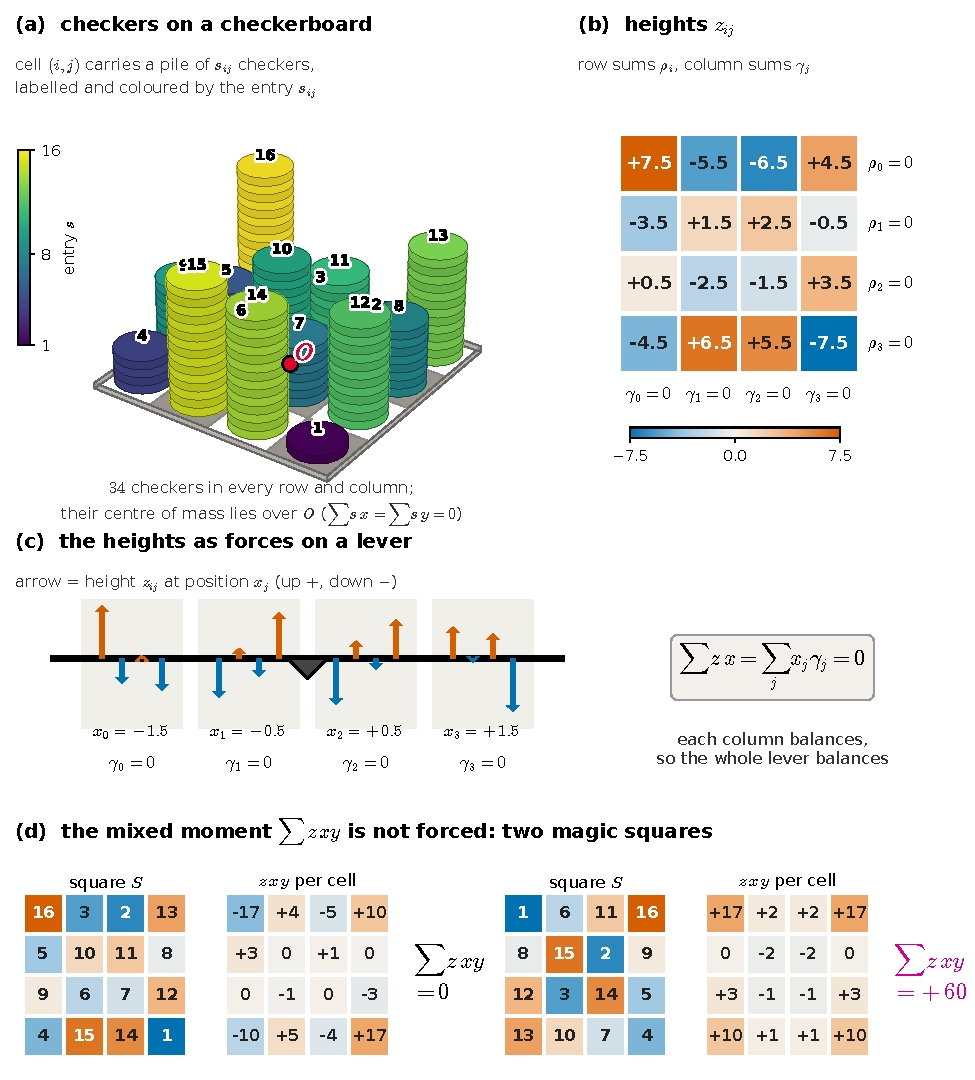
\includegraphics[width=0.86\textwidth]{figures/fig_moments.pdf}
\caption{(a)~D\"urer's square as piles of checkers, $s_{ij}$ on cell $(i,j)$, seen from the front of the board in the orientation of the square; each row and column carries $34$ checkers, so their centre of mass lies over the centre $O$. (b)~The mixed moment: for D\"urer's square and for square \#45 the integers $8\,z\,x\,y$ per cell; they sum to $0$ and to $480$.}
\label{fig:moments}
\end{figure}

\begin{figure}[htbp]
\centering
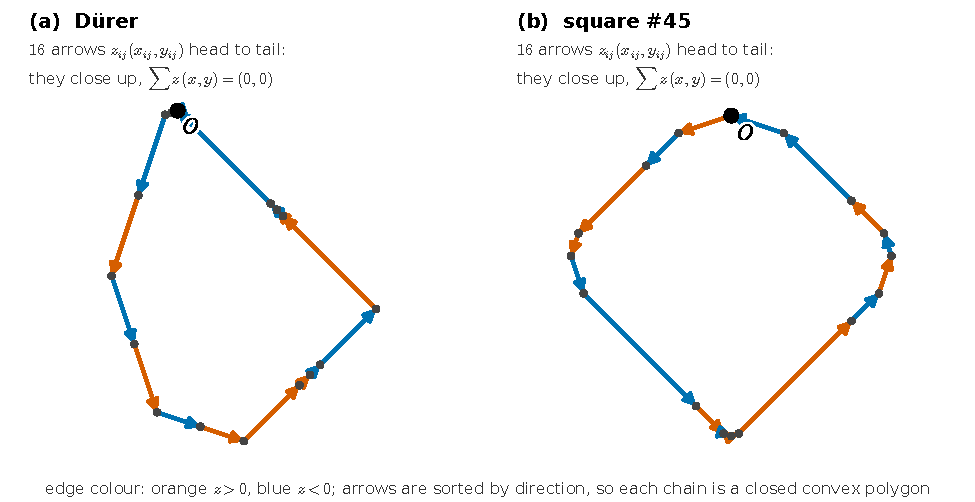
\includegraphics[width=0.86\textwidth]{figures/fig_weighted_sum.pdf}
\caption{The dipole moment $\sum z_{ij}\,(x_{ij},y_{ij})$ for D\"urer's square and square \#45 (\Cref{fig:moments}b): the $16$ vectors $z_{ij}(x_{ij},y_{ij})$ (orange for $z>0$, blue for $z<0$), sorted by direction and laid head to tail, close up at $O$. The tables give $\sum z\,xy$ over the four quadrants of the grid; the totals are $0$ and $60$.}
\label{fig:weighted}
\end{figure}
